\chapter{Background \& Related Work}\label{C:background}

This chapter explains the background and literature of recommender system techniques. It firstly explores content-based filtering, and then explores collaborative filtering.

\section{Content-based Filtering}
\todo{redo this}
Content-based filtering has been widely used in recommender systems. Content-based filtering focuses on recommending items to a user based on the attributes and content of items corresponding to the attributes a user has explicitly or implicitly liked. Content-based filtering techniques may involve extracting information from the user to create a profile of attributes the user implicitly likes. Pandora, a music streaming station automatically plays recommended songs that the user may enjoy as soon as the user has indicated a song they have liked \todo{reference this shit}. The recommendations are based on \todo{400} attributes of a song, and are extracted from the user as soon as they have liked a song. However, content-based filtering is prone to recommending only a small subset of items, since it recommends items based on attributes of the items, leading to overspecialisation and thus, restricting variety \cite{toward}. Another problem of content-based filtering is that it may be difficult to extract features from items and users, and manually labelling these features may not be practical \cite{toward}.

Traditional collaborative filtering explained in the following sections, are able to address these concerns since attributes are ignored, and recommendations are based on actions of other users, providing a range of recommendations that are not restricted to specific attributes \cite{koren2009matrix}. However, in the ``Cold Start" problem, content-based filtering is superior than collaborative filtering because it does not rely on the opinion of other users \cite{koren2009matrix}.

For these reasons, we do not address content-based filtering in detail, but explain the basic idea of content-based filtering since hybrid collaborative filtering approaches use it. The following sections explain the details of collaborative filtering.  

\section{Collaborative Filtering}

Collaborative filtering (CF) is a popular technique that has been successfully used in recommender systems \cite{itembased, schafer2007collaborative, survey}. The main idea behind collaborative filtering is that rating behaviours of others can be used to predict items that the active user will be interested in. Intuitively, this algorithm stems from the assumption that users having similar opinions on items they both rated tend to have similar tastes to each other, having similar opinions about other items  \cite{schafer2007collaborative}. For example, consider a friend with whom you share common food interests. Perhaps you both like eating chicken sandwiches. Since you and your friend have similar tastes, your friend may then be able to suggest to you another food dish that you might enjoy such as Thai Green Curry. Collaborative filtering uses the same concept, but usually on a larger scale. 

\begin{figure}
\centering
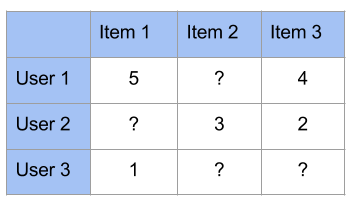
\includegraphics[scale=0.7]{images/User-Item}
\caption{A user-item ratings matrix containing scaled ratings from 1-5. Typically the user-item ratings matrix is sparsely filled, since there will be missing entries where users have not rated a subset of items. The missing entries are represented by the question marks (?) in the matrix. }
\label{fig:matrix}
\end{figure}

Users express their preferences for a variety of items through ratings which can be in various forms such as 1-5 star ratings, or binary scale ratings such as likes/dislikes. These ratings are typically represented as a (User, Item, Rating) triplet. These ratings can be represented in the form of a matrix, where the rows of the matrix are users, the columns of the matrix are items, and the ratings are represented inside the matrix (See Figure \ref{fig:matrix}). Since the matrix contains sets of rating triplets, the (User, Item) pairs will exist where a user has not yet rated the item, thus the matrix is usually sparse.

Since the matrix can be sparse, collaborative filtering can struggle when there are not enough ratings to provide accurate recommendations to users. Sparse ratings can also lead to another issue called the 'Cold Start' problem, where ratings for new items or new users have not yet been collected. In this context, content-based filtering is superior \cite{koren2009matrix}. However, the advantage of collaborative filtering is that it does not require domain knowledge of items or users to provide recommendations. It focuses on the previous behaviours of users and their rating history, providing recommendations that are generally more accurate than content based filtering once the active user has rated enough items \cite{koren2009matrix, schafer2007collaborative}. 

Using the matrix, a list of top N recommendations is usually given to the user representing the items they will like, computed through collaborative filtering techniques. For example, the active user may be recommended 10 food dishes that might be of interest to them whenever they log onto the application What's On The Menu (WOTM) specified in Section \ref{section:wotm}.  

There are three main areas of CF, these areas are memory-based CF techniques, model-based CF techniques, and hybrid-based CF techniques. In this project, we will be examining in particular, the neighbourhood methods which are a form of memory-based CF techniques, and latent factor models which are a form of model-based CF techniques \cite{survey, koren2009matrix}. Neighbourhood methods, and Latent factor models will be explained in the following sections. 

% \section{Challenges}
% \subsection{Cold Start}
% \subsection{Data Sparsity}
% \subsection{Synonyms}
% \subsection{Scalability}
% \subsection{Grey Sheep}
% \subsection{Shilling attacks}
% \subsection{Diversity and the Long Tail}

\section{Neighbourhood Methods}

Neighbourhood CF methods can be classified into the class of memory-based CF techniques because they use the entire or a sample of the ratings matrix to find the similarity between users (or items) through a heuristic \cite{memorybased, schafer2007collaborative}. The main idea of this approach is to use the ratings matrix to compute the similarity between users (or items) which are then used for recommendations. This typically involves finding all user-user similarities (or item-item similarities) and using neighbourhood algorithms such as K-Nearest Neighbour to find the K most similar users (or items), referred to as neighbours. The K most similar users (or K most similar items) are then used to predict how the active user will feel about specific items, thus being able to make recommendations for the active user based on their neighbours. Since these neighbours may contain quirky characteristics that are not common among the users, methods tend to take the weighted average of the neighbours ratings or simple weighted average to generate predictions for the active user \cite{survey}. 

Common similarity measures that are used are Pearson's Correlation, Cosine similarity, Euclidean distance, Jaccardian similarity and so forth, finding similar users to the active user (or similar items that the active user has previously performed actions on). The most common neighbourhood method that is used to find the most similar users (or items) is the K-Nearest Neighbour algorithm. This algorithm finds the K-nearest neighbours based on a heuristic, in this case, the similarity measure. Other neighbourhood algorithms are K-Means, K-d Trees, and Locality Sensitive Hashing \cite{survey}. 

% A key problem of collaborative filtering is how to combine and weight the preferences of user neighbors. Sometimes, users can immediately rate the recommended items. As a result, the system gains an increasingly accurate representation of user preferences over time.

The following section explains the difference between user-based CF and item-based CF.

% +Advantages
%     -   explain
%     - easy to create etc
%     - easy facilitation of new data
%     - content independence of itemsbeing reocmmended
%     - good scaling with co-rated items
% +Disadvantages
%     - performance decrease with sparse data
%     - scalability and problems with large datasets
%     - adding new items required inclusion of the new item and re-insertion of all elements in the structure



\subsection{User-based Collaborative Filtering}

The defining characteristic of user-based CF is based upon similarities between users \cite{mahoutaction}. A concrete example would be two users that rated the same food dishes similarly, the first user has indicated that they like the Big Mac and the Whopper Burger; similarly, the second user indicated that they like the Big Mac too, therefore, since these two users previous ratings are similar (both like Big Macs), they are to be considered similar; we can then recommend to the second user that they should try the Whopper Burger, since the users have similar opinions about the item. User-based CF has the same idea with the example, but typically works better on a larger scale - more ratings, more users, and more items are involved. 


\subsection{Item-based Collaborative Filtering}

Another approach that is commonly used is Item-based CF. Instead of finding users that are similar to each other, item-based CF focuses on recommending items that are similar \cite{mahoutaction}. Similar items are extracted by the rating patterns of other users rather than the attributes of the item - two items are considered similar if users rate them similarly \cite{schafer2007collaborative}. For example, a user could have previously liked the following dishes: a chicken sandwich, chicken nuggets, and chicken soup. Item-based CF will find similar items that the user has previously rated by using a similarity measure. By using this technique, it may recommend items based on the users previous interests, suggesting new items such as chicken salad, or a chicken burger since users who like the previous dishes of the active user tend to like these dishes. This is the main idea behind item based collaborative filtering. 


\section{Latent Factor Models}


% \textcolor{red}{
% Latent factor models, such as matrix factorization (aka, SVD), comprise
% an alternative approach by transforming both items and users to the same latent factor
% space. The latent space tries to explain ratings by characterizing both products
% and users on factors automatically inferred from user feedback \cite{koren2011}
% }

Latent factor models can be classified into the class of model-based CF techniques because they try and explain ratings by automatically inferring meaningful information from users previous rating patterns which are then used to make intelligent predictions based on this meaningful information \cite{survey}. For example, these methods automatically try and learn about the properties or characteristics of the items such as the food dishes, and learn how much the user likes each of these properties, also known as latent factors \cite{koren2011}. 

Matrix factorization is seen as one of the successful techniques of latent factor models \cite{memorybased, koren2009matrix}. Singular Value Decomposition is a matrix factorization technique that is well-known and can be applied to the CF domain, identifying latent semantic factors \cite{koren2009matrix}. The following section talks about the matrix factorization technique of Singular Value Decomposition and how it is used to recommend items to users. 

%  These methods have become popular in
% recent years by combining good scalability with predictive
% accuracy. In addition, they offer much flexibility for modeling
% various real-life situations

\subsection{Matrix Factorization}

\todo{Fix this section - explain that it only maps to rated items}

In the context of this project, the main goal of Singular Value Decomposition (SVD) is to train a model to learn what properties of a dish that a user likes. This can be used to predict how a user may feel about another dish by looking at the properties that are inferred from that dish.
\todo{Clarification about the context of SVD - From Simon Funk and not mathematical one.}


SVD decomposes the ratings matrix, where both users and items are mapped to a joint latent factor space of dimensionality \begin{math} f \end{math} - the space containing the inferred properties of the food dishes, and how the users feel about those properties. The latent space tries to explain the ratings given from the ratings matrix by considering these inferred latent factors. These latent factors are represented in the form of an item vector \begin{math} q_{i} \in \mathbb{R}^f  \end{math} and a user vector \begin{math} p_{u} \in \mathbb{R}^f  \end{math} where \begin{math} i \end{math} is a given item and \begin{math} u \end{math} is a given user. The vectors contain a specified number of factors for each item and user, which are used to predict how the user may feel about other items that they have not yet rated \cite{koren2009matrix}. Factors in the item vectors could be dimensions regarding the properties of the items. An example for food dishes are item vectors that discover factors measuring obvious dimensions in the food dish such as the ingredients, spice levels, cuisine type, or meat type; less defined dimensions such as carbohydrates, or uninterpreted dimensions in the food dish \cite{koren2009matrix}. User vectors contain factors that measure the extent that the user likes those factors which are the properties that are inferred from the food dishes \cite{koren2009matrix}. These factors in \begin{math} q_{i} \end{math} and \begin{math} p_{u} \end{math} can be positive or negative, representing how much the properties contained within each dish, and how much the user likes those properties. 

These feature vectors contain a specified number of factors for each item and user, which are used to predict how the user may feel about other items that they have not yet rated \cite{koren2009matrix}. For this model, a user's predicted rating for a dish would be the dot product of the food dish vector, and the user vector \begin{math} q_{i}^T p_{u} \end{math}. This approximates to the active user's rating of the current item, denoted by \begin{math} r_{ui} \end{math}, leading to the estimate \cite{koren2009matrix}

\begin{equation}\label{eq:1}\tag{1} \widehat{r} = q_{i}^T p_{u} \end{equation}.

% \begin{equation}\label{}

Since the user vector represents how much they like about the characteristics of the dish, and the item vector represents the portion of how much of the dish contains those properties \cite{koren2009matrix}, we can use the dot product - multiplying the dish containing a specific property from the item vector with how much the user likes that property from the user vector, and repeat this for all elements in the vectors to see the overall interest that the user has of the dish. This represents the active user's interest about the overall dish and is used to estimate the rating a user will give to the item. 

% Now that we understand how the predicted ratings for an item and user are computed, you may be wondering how we infer the item and user vectors explained above. 

To infer the item and user vectors explained above, the system learns the model by fitting the previously observed ratings. However, directly modelling the observed ratings can lead to over fitting, being overspecialized leading to inaccurate future predictions.

To prevent this, the idea is to use a regularized model that is used to generalize the previous ratings in a way that is able to predict future unknown ratings. To learn the vectors for the items and users, the system uses an equation that minimizes the regularized squared error on the set of known ratings.

\begin{equation}\label{eq:2}\tag{2}
\displaystyle min_{q*,p*} \sum_{ (u,i) \in K} (r_{ui} - q_{i}^T p_{u}) + \lambda (\| q_{i} \|^2 + \| p_{u} \|^2 )
\end{equation}

\begin{math} K \end{math} represents the training set from the rating matrix where \begin{math} r_{ui} \end{math} is known for the user, item pairs \begin{math} (u,i) \end{math}. The constant \begin{math}\lambda\end{math} controls the regularization used to penalize the magnitudes to avoid over fitting, and is typically tuned by cross-validation. Minimization is performed by Alternating Least Squares \cite{koren2011}  which is detailed below. 

% In order to fill in these missing values, singular value decomposition is used to learn feature vectors (factors) of items and users. The items feature vectors represent the characteristics of the items, in this case: dishes. User feature vectors represent how much the user prefers these characteristics of the dish. However, since the user item matrix contains many missing values it is unwise to train directly from it, as it is highly to cause overfitting. You can use inductions? to fill in these will values, but it takes up space, and may cause a lot of error if you get it wrong. Therefore you use the ratings given, but use lambda to determine the strength of those ratings. From there you can learn these algorithms. 

% Now you may be wondering how these feature vectors are learnt. These feature vectors are learnt through an equation, in which we minimise the square error to find the best latent features. By doing this, we use two algorithms to find the minimum error and to find the appropriate feature vectors.

\subsubsection{Alternating Least Squares} \label{als}

The main purpose of Alternating Least Squares (ALS) is to find the minimum error from equation \ref{eq:2}, which is used to learn the factors in each of the vectors based on the rating matrix. ALS works to find the item and user vectors by initializing the vectors with random values depending on how many factors are specified. From this, it fixes values of one of the vectors first such as the item vector, then computes and reassigns values of the user vector according to the minimization equation, shown as equation \ref{eq:2} above. After this, it alternates - the user vector values are now fixed, and the re-computation of the item feature values occur, trying achieve the result of the smallest value for the minimization equation. This technique keeps alternating between fixing the vector values, until there is a convergence where the values in the two vectors no longer change the minimization equation, or there are minimal changes, hence the name Alternating Least Squares. This is used to find the minimum error from the equation mentioned above and to learn the factors in each of the vectors. 

\todo{Why do I choose this? Report results from literature}

\subsection{Hybrid-based Collaborative Filtering}
\todo{Consider redoing this}
For traditional collaborative filtering techniques, they mainly suffer from the cold start problem from the sparsity of ratings in the user ratings matrix \todo{reference}. Matrix factorization techniques also may suffer from problems such as the curse of dimensionality \todo{Curse of dimensionality?}. Content-basd filtering techniques generally provide good recommendations, and are superior in this context, however, suffer from providing recommendations that are predictable and are restricted to content that is similar, thus, making factors such as novelty or serendipity non-existent. For these reasons, hybrid collaborative filtering approaches have been used. There are many approaches to hybrid-collaborative filtering approaches, but typically range from using collaborative filtering and content-based filtering in order to alleviate the disadvantages, and complement instead. The following are techniques which can be found in \todo{cite the link yo. What about binary choices??}
\subsubsection{Mix and Match}
\subsubsection{Content-boosted filtering}
\subsubsection{Switch}
\todo{yadadadada}

\section{Literature Review \& Applications}

The term 'collaborative filtering' was first introduced in \citeyear{goldberg1992using} by \citeauthor{goldberg1992using} to describe the technique used in Tapestry, one of the earliest known recommender systems \cite{koren2009matrix,  goldberg1992using, itembased, survey}.

Tapestry \cite{goldberg1992using} was created to handle electronic documents and used manual collaborative filtering, allowing users to query information based on other's opinions about the documents. These opinions were in the form of annotations or replies which users were encouraged to make on documents to increase probability of relevant results returned from queries \cite{schafer2007collaborative}. Tapestry relied on opinions from a small community such as an office workgroup, where each person's opinion was trusted. Larger communities could not rely on every person knowing each other, leading to new collaborative filtering techniques being developed \cite{itembased}. 

\todo{ADD THIS AS MOTIVATION FOR BACKGROUND}
More recommender systems emerged as value was seen in the potential to increase sales from recommendations - customers may purchase suggested items that they might not have seen otherwise \cite{schafer2007collaborative}. Perhaps the most popular recommender system in the late 1990's was used in Amazon.com, collecting user purchase history, browsing history, and recently viewed items to recommend items that the user may buy \cite{schafer2007collaborative}. Other recommender systems consisted of Jester \cite{goldberg} for jokes, and Ringo \cite{ringo} for music.
% /cite{schafer2007collaborative, toward}
GroupLens \cite{grouplens} were the first to introduce a neighbourhood collaborative filtering technique. Building upon the Tapestry concept, GroupLens created an automated user based collaborative filtering technique for recommending Usenet articles that users may be interested in. The advantage of neighbourhood methods is that they are intuitive, easy to implement, and produce highly effective results \cite{survey, scalable}. Despite providing accurate recommendations, user-based collaborative filtering techniques were computed in real time and their performance would degrade as more users and items were added to the system, leading to scalability and performance issues \cite{dimension, itembased, evaluationitem}.

\todo{Remove this?}
This required collaborative filtering techniques that could easily scale and still produce high quality recommendations, leading to the exploration of item-based collaborative filtering. Item-based collaborative filtering techniques were developed to address scalability limitations of the user-based techniques \cite{survey}. \citeauthor{itembased} analyzed various item-based recommendation algorithms, computing item-item similarities and comparing the accuracy with traditional KNN user based collaborative filtering techniques \cite{itembased}. \citeauthor{itembased} found that items remained fairly static in the system, whereas user behaviours and preferences would often change. Because items were found mostly static, it meant precomputation could occur for item similarities. By having precomputed item similarities, traditional item-based collaborative filtering can then be applied, thus performance and scalability would be increased \cite{scalable}.

Other techniques such as model based collaborative filtering have also been investigated to overcome the performance and scalability issues. Well known model based techniques include Bayesian belief nets \cite{baysian}, clustering models \cite{clustering}, and latent semantic models \cite{latent}. These models are based on learning patterns from users previous actions to predict new items, and are expensive but can be built offline allowing high scalability. The resulting model is ``very small, very fast, and essentially as accurate as nearest neighbor methods" \cite{itembased}. \citeauthor{itembased} found Bayesian networks to be practical in the context where user ``preferences change slowly with respect to the model" \cite{itembased}. However, these models are not suitable for environments where the user preference model should be updated rapidly or frequently. Since model based approaches do not have to compute similarity measures to form neighbourhoods, they tend to produce faster recommendations and outperform neighbourhood models in terms of accuracy of recommendations \cite{toward, itembased}. 

Although collaborative filtering is considered to be one of the most successful approaches to recommender systems \cite{survey, toward}, they suffer from the problem of data sparsity \cite{toward, survey, itembased, koren2009matrix, koren2011, dimension}. Data sparsity is when only a small subset of user ratings on items are recorded, leading to an insufficient number of ratings to produce accurate recommendations. Data sparsity specifically tends to appear in the 'cold start' problem, where new items or new users are entered into the system, but not enough information is supplied to produce accurate recommendations since recommendations are based on common items or users \cite{survey}.

To alleviate this problem, hybrid approaches were investigated that combined collaborative filtering and other recommender techniques such as content based filtering. \citeauthor{toward} suggested creating user profiles such that demographic information could be included in similarity measures to provide extra content to find similar users or items. This effectively makes use of content-based filtering where recommendations are produced based on the content and attributes of the items, learning what attributes the user likes \cite{toward}. Well-known hybrid techniques include content-boosted collaborative filtering \cite{hybrid}, and personality diagnosis \cite{hybrid2, survey}. Hybrid approaches were implemented to address the limitations of collaborative filtering and content-based filtering techniques \cite{toward}, but have increased complexity leading to more expensive computations. Additionally, external information is needed about the content of the items which may not be available, thus making hybrid approaches impractical in certain scenarios \cite{survey}. \citeauthor{dimension} found a different approach that used dimension reduction techniques such as Singular Value Decomposition, making sparse rating models more dense by reducing the dimensionality of the product space, thereby condensing the modelled ratings of users and producing less missing information \cite{dimension}. 

In 2006, the Netflix Prize competition attracted interest in the field of recommender systems \cite{survey}. Netflix offered a \$ 1 million dollar prize to the first team to improve their movie recommender system by 10\%. This attracted interest in the research field of recommender systems. The team ``BellKor in Pragmatic Chaos" won the competition in 2009 basing their solution on a combination of latent factor models and neighbourhood models \cite{winning, survey}. These models took into account many biases which improved the predication accuracy. \citeauthor{koren2009matrix} were part of the winning team, and wrote a paper explaining how temporal effects, and user biases could be accounted for in latent factor models such as Singular Value Decomposition, making it superior to neighbourhood methods because of its flexibility \cite{koren2009matrix}. \citeauthor{koren2011} later published a paper about their findings and solutions to the Netflix Prize competition in \cite{koren2011} and \cite{winners}.

\todo{What about related food recommendation systems? Positives?, Negatives?}

\section{Requirements / Discussions}

\todo{Fix - talk about how SVD is good for sparse data?}

Existing research focuses on the scalability and prediction-accuracy of these collaborative filtering techniques. Literature suggests that latent factor models such as SVD produce better prediction-accuracy and solve the scalability issue \todo{cite this, and state that incremental SVD is scalable}. Since SVD is a model-based CF technique, it means expensive computation can be done offline, training the model. When the model is already trained, the performance of recommendations will be fast \todo{explain dot product} since precomputation has already occurred offline. This makes a model-based SVD approach the top candidate for our food recommendations application WOTM. 

However, model-based approaches need to be updated frequently. In terms of scalability, WOTM is expected to contain a much smaller number of users or items as existing recommender systems used by Netflix, Facebook, and Google. For this reason, neighbourhood methods may be a good choice, as they provide the ability to explain the reasoning behind the recommendations, as well as give good prediction-accuracy results. Scalability should not be a top concern with this application. Therefore, real time computation may be a factor to consider. Therefore, this method also needs to be explored to see if it is suitable for WOTM.

It is evident that there has been an abundance of existing research on collaborative filtering techniques and ways to improve the prediction accuracy. However, \citeauthor{schafer2007collaborative} states these factors alone, do not contribute to making a good recommender system \cite{schafer2007collaborative}. Instead, \citeauthor{schafer2007collaborative} states that recommendation is not a ``one-size-fits-all problem"  \cite{schafer2007collaborative}. Specific tasks, information needs, and item domains represent unique problems for recommenders, and design and evaluation of recommenders needs to be done based on the user tasks to be supported" \cite{schafer2007collaborative}. Similarly, \citeauthor{martin2009recsys} argues that the recommender algorithm is only one factor from many for providing recommendations to users. \citeauthor{martin2009recsys} explains that the user experience, data collection, and other problems which make up the whole of the recommender experience need to be considered \cite{schafer2007collaborative, martin2009recsys}. \citeauthor{interface} concluded in \cite{interface} that much of the accuracy problem has been solved in recommender systems, however delivering these accurate predictions to users in a way that creates the ``best experience for them remains an open problem" \cite{interface}. 

For this reason, this project focuses on the goal of providing a recommender system that fits the needs for the ``What's On The Menu" application. This involves considering how users ratings will be collected, the user experience, the recommendation process, and what factors are considered to be important in the recommendation process such as the trade-offs between scalability, prediction accuracy, and performance.

A focus on the recommender system will be on how to make the user experience as easy as possible for users. The user experience affects the collection of ratings from users and the frequency in which users will rate food dishes, thus affecting the quality of recommendations. Another focus will be on the performance of providing recommendations to the users. \todo{Keep? In this case, prediction accuracy may be less important than the speed/performance of recommendations being produced.} If the recommendation process is slow, users are less likely to continue using the application. On the other hand, if prediction accuracy is not accurate, then users will be recommended items that may not be of interest. A fair trade-off must be considered. 

\todo{Feedback from examiner}
\todo{
Regarding section 4.1. about performance vs prediction accuracy, there were some essays discussing the results of the Netflix challenge; I believe (please check) the conclusion was that very simple methods such as SVD work well when there is enough data. Performance and accuracy are not contrary goals in this case - high performance is needed to deal with large amounts of data; the O(N\^3) scaling of a standard SVD would not work. I believe the methods that won the challenge were similar to SVD, but with a performance that was cubic in the rank rather than the number of data points. 
}

% In terms of scalability, the "What's On The Menu" application is not particularly expected to contain anywhere near the number of users or items as existing recommender systems used by Netflix, Facebook, and Google. For this reason, neighbourhood methods may be a good choice, as they provide for the ability to explain the reasoning behind the recommendations, as well as give good prediction-accuracy results. Scalability should not be a top concern with this application. Therefore, real time computation may be a factor to consider.


% In terms of scalability, the "What's On The Menu" application is not particularly expected to contain anywhere near the number of users or items as existing recommender systems used by Netflix, Facebook, and Google. For this reason, neighbourhood methods may be a good choice, as they provide for the ability to explain the reasoning behind the recommendations, as well as give good prediction-accuracy results. Scalability should not be a top concern with this application. Therefore, real time computation may be a factor to consider.

% + main challenges, sparsity \cite{survey, dimension}, scalability, synonymy \cite{dimension}, gray sheep, shilling attacks, privacy protection, etc \cite{survey}.

% \section{Representational State Transfer (REST)}

% REST stands for REpresentational State Transfer. REST is an architectural style for building a software application that can be used to communicate to other systems through the HTTP protocol. It uses resources to represent important data that can be retrieved by other systems via methods from the HTTP Protocol (GET, POST, PUT, DELETE etc). It utilizes a client-server, and is stateless in the sense that all the data that is needed is sent through the HTTP protocol to the other system.

% \section{Application Program Interface (API)}

% API stands for Application Program Interface. An API describes the methods and ways in which others can interact and use these tools to build software applications. It specifies how software components should interact and how the software methods, or services behave. 

% This truncation simultaneously achieves two goals. First, it decreases the dimensionality of the vector space, decreasing the storage
% and computational requirements for the model. Items and users can each be represented by k-dimensional vectors. Second, by dropping
% the smaller singular values, small perturbances as a result of noise in the data are eliminated, leaving only the strongest effects or trends in the model. In collaborative filtering, this noise can come as a result of other factors besides sheer preference playing a role in a user’s rating;
% decreasing the impact of noise improves our ability to provide highquality
% recommendations.

% Singular value decomposition is only well-defined when the matrix
% is complete. Therefore, to factor the ratings matrix, the missing values
% must be filled with some reasonable default (a method called imputation).
% Sarwar et al. [131] found the item’s average rating to be a
% useful default value (they tried user average as well, but item average
% performed better). Alternatively, the SVD can be computed over the
% normalized ratings matrix Rˆ (see Section 2.1) and the missing values
% considered to be 0.
% Several methods have been proposed that compute an estimate
% of the SVD only on the known ratings, dropping the requirement to
% impute or otherwise account for missing ratings. Kurucz et al. [81]
% propose a least-squares method that learns a regression for each user.

% Once the SVD is computed, it is necessary to update it to reflect
% new users, items, and ratings. A commonly used method for updating
% the SVD is folding-in; it works well in practice and allows users who
% were not considered when the ratings matrix was factored to receive
% recommendations and predictions [16, 129]. Folding-in operates by computing
% a new user-preference or topic-relevance vector for the new user
% or item but not recomputing the decomposition itself. 

% Setting the unknown ratings to 0 caues folding-in to ignore them, and a new user preference vector is now available. As user and item vectors are updated with the folding-in process, the
% accuracy of the SVD will diminish over time. It is therefore necessary
% to periodically re-compute the complete factorization. In a deployed
% system, this can be done off-line during low-load times [129].
% Brand [21] proposed an alternative method for building and maintaining
% the SVD based on rank-1 updates. His method produces fast,
% real-time updates of the SVD, bootstrapping the SVD with a dense
% portion of the data set. This dense portion can be extracted by sorting
% users and items to make a dense corner in the ratings matrix.
